% Copyright (c) 2016-2020 The ALF project.
% This is a part of the ALF project documentation.
% The ALF project documentation by the ALF contributors is licensed
% under a Creative Commons Attribution-ShareAlike 4.0 International License.
% For the licensing details of the documentation see license.CCBYSA.

% !TEX root = doc.tex


ALF includes modules providing predefined structures which the user can combine together or use as templates for defining new structures, namely: 
\begin{itemize}
	\item lattices and unit cells -- \texttt{Predefined\_Latt\_mod.F90}
	\item hopping Hamiltonians -- \texttt{Predefined\_Hop\_mod.F90 }
	\item interaction Hamiltonians -- \texttt{Predefined\_Int\_mod.F90}
	\item observables -- \texttt{Predefined\_Obs\_mod.F90 }
	\item trial wave functions -- \texttt{Predefined\_Trial\_mod.F90 }
\end{itemize}
which are defined using the data structures defined in the Sec.~\ref{sec:imp}, as described in this section.



%%%%%%%%%%%%%%%%%%%%%%%%%%%%
% !TEX root = doc.tex
% Copyright (c) 2017-2020 The ALF project.
% This is a part of the ALF project documentation.
% The ALF project documentation by the ALF contributors is licensed
% under a Creative Commons Attribution-ShareAlike 4.0 International License.
% For the licensing details of the documentation see license.CCBYSA.
%
%-----------------------------------------------------------------------------------
\subsection{Predefined lattices} \label{sec:predefined_lattices}
%-----------------------------------------------------------------------------------


The types \texttt{Lattice} and \texttt{Unit\_cell}, described in Section~\ref{sec:latt}, allow us to define arbitrary one- and two-dimensional Bravais lattices. The subroutine \texttt{Predefined\_Latt} provides some of the most common lattices, as described bellow.


\begin{figure}
        \begin{center}
                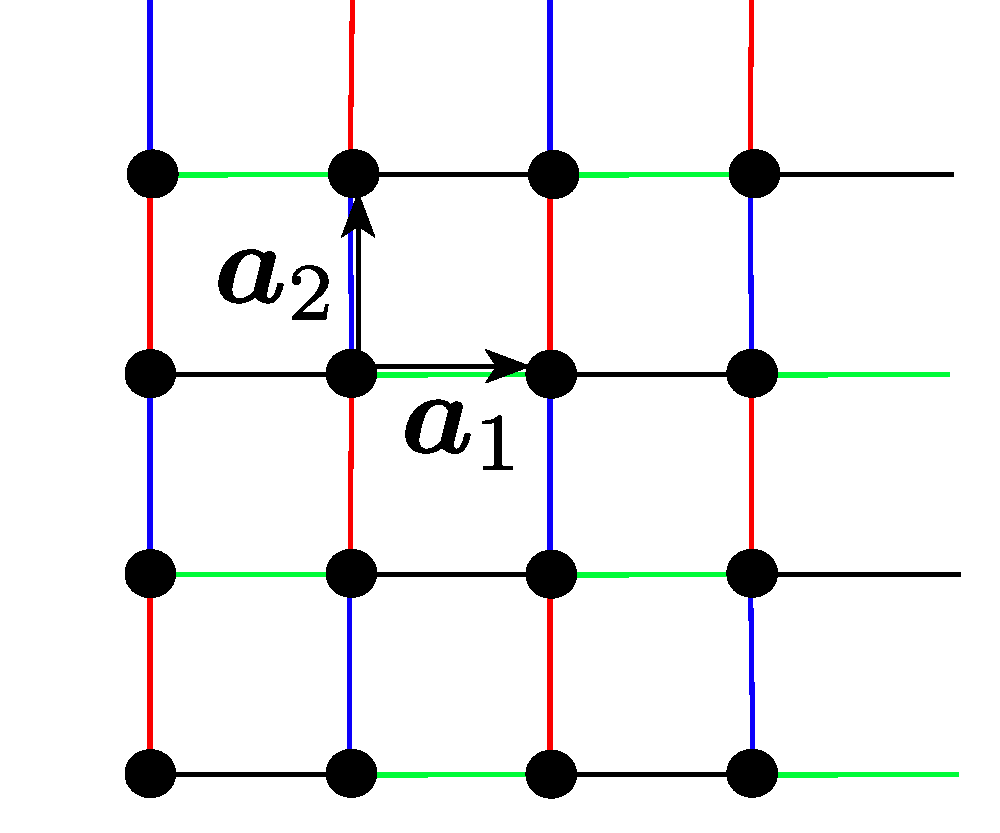
\includegraphics[width=.3\textwidth]{Figures/Square.pdf}
                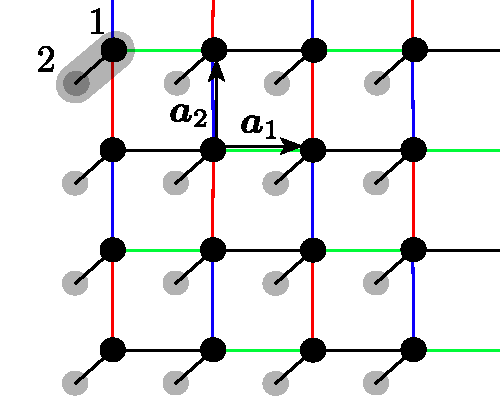
\includegraphics[width=.3\textwidth]{Figures/Square_bilayer.pdf} 
                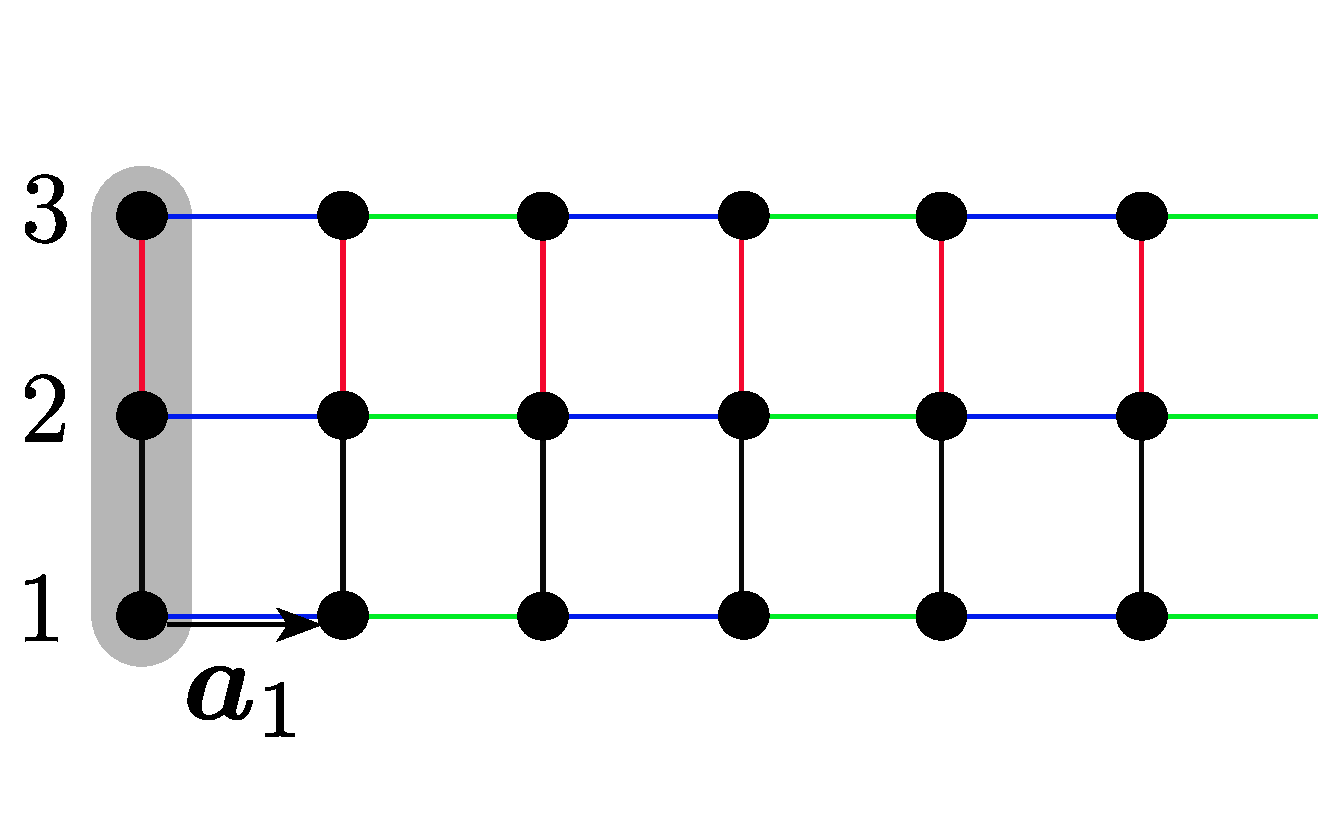
\includegraphics[width=.3\textwidth]{Figures/N-Leg-Lad.pdf} \\
                 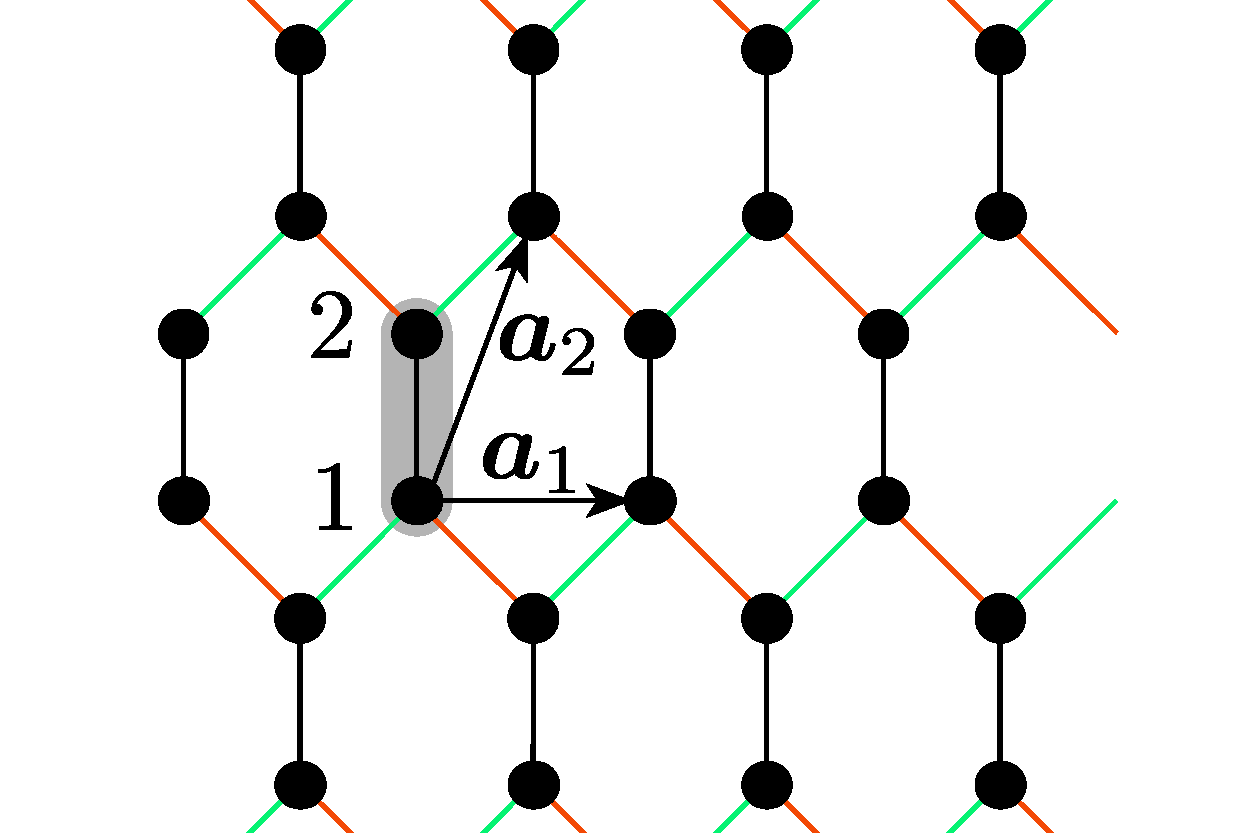
\includegraphics[width=.4\textwidth]{Figures/Honeycomb.pdf} 
 		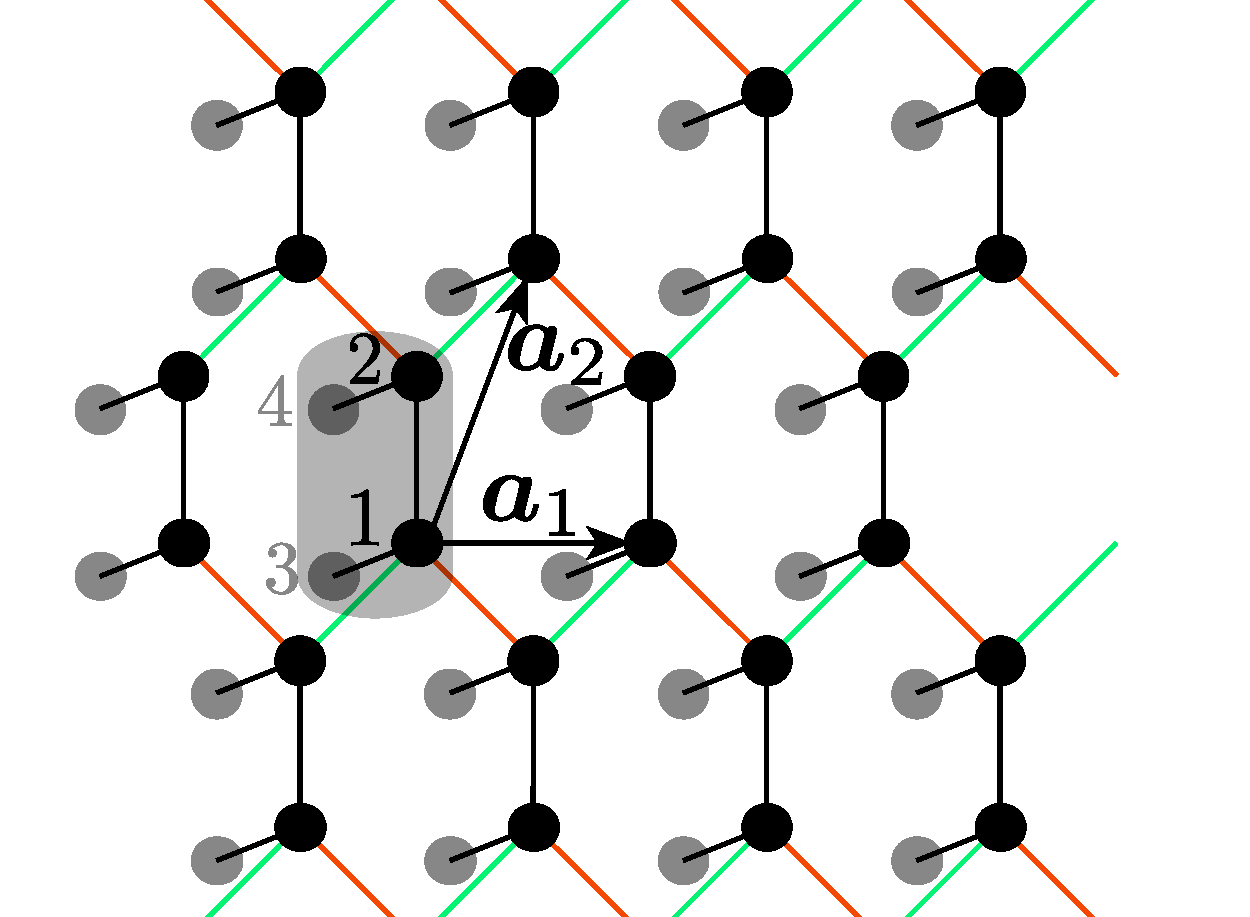
\includegraphics[width=.4\textwidth]{Figures/Honeycomb_bilayer.pdf}
				
                \caption{}
                \label{fig_predefined_lattices}
        \end{center}
\end{figure}


The subroutine is called as:
\begin{lstlisting}[style=fortran]
Predefined_Latt(Lattice_type, L1, L2, Ndim, List, Invlist, Latt, Latt_Unit)
\end{lstlisting}
which returns a lattice of size \texttt{L1$\times$L2} of the given \texttt{Lattice\_type}, as detailed in Table~\ref{table:predefined_lattices}. Notice that the orbital position \texttt{Latt\_Unit\%Orb\_pos\_p(1,:)} is set to zero unless otherwise specified.
%
\begin{table}[h]
	\begin{center}
	\begin{tabular}{@{} p{0.13\columnwidth}  p{0.1\columnwidth} p{0.09\columnwidth} p{0.58\columnwidth}  @{}}
		\toprule
		Argument                 & Type       & Role   & Description \\
		\midrule
		\texttt{Lattice\_type}   & String     & Input  & lattice configuration, which can take the values:
		\vspace{-\topsep} %sometimes dispensable
		\begin{itemize}
			\setlength{\itemsep}{0pt} \setlength{\parskip}{0pt} \setlength{\parsep}{0pt}
			\item[-] \texttt{Square}
			\item[-] \texttt{Honeycomb}
			\item[-] \texttt{Pi\_Flux}  (deprecated)
			\item[-] \texttt{N\_leg\_ladder}
			\item[-] \texttt{Bilayer\_square}
			\item[-] \texttt{Bilayer\_honeycomb}
			\vspace{-1.4\topsep} 
		\end{itemize} \\
	    %\vspace{-\topsep} \\ \vspace{-\topsep}
		\texttt{L1}, \texttt{L2} & Integer    & Input  & lattice sizes (set \texttt{L2=1} for 1D lattices)\\
		\texttt{Ndim}            & Integer    & Output & total number of orbitals\\
		\texttt{List}            & Integer    & Output & for every site index $\texttt{I} \in [1,\texttt{Ndim}]$, stores the corresponding lattice position, \texttt{List(I,1)}, and the (local) orbital index, \texttt{List(I,2)}\\
		\texttt{Invlist}         & Integer    & Output &  for every $\texttt{lattice\_position} \in [1,\texttt{Latt\%N}]$ and $\texttt{orbital} \in [1,\texttt{Norb}]$ stores the corresponding site index \texttt{I(lattice\_position,orbital)}\\
		\texttt{Latt}            & Lattice    & Output &  sets the lattice\\
		\texttt{Latt\_Unit}      & Unit\_cell & Output & sets the unit cell\\
		\bottomrule
	\end{tabular}
\caption{Arguments of the subroutine \texttt{Predefined\_Latt}.   Note that the Pi\_Flux lattice is deprecated for the moment since it can be emulated with the Square lattice with half a flux quanta piercing each plaquette.}		\label{table:predefined_lattices}
\end{center}
\end{table}

In order to easily keep track of the orbital and unit cell, \texttt{List} and \texttt{Invlist} make use of a super-index, defined as shown below:
\begin{lstlisting}[style=fortran]
nc = 0                                  ! Super-index labeling unit cell and orbital
Do I = 1,Latt%N                         ! Unit-cell index 
   Do no = 1,Norb                       ! Orbital index
      nc = nc + 1
      List(nc,1) = I                    ! Unit-cell of super index nc
      List(nc,2) = no                   ! Orbital of super index nc
      Invlist(I,no) = nc                ! Super-index for given unit cell and orbital
   Enddo
Enddo
\end{lstlisting}
With the above lists one can run through all the orbitals and at each time keep track of the unit-cell and orbital index. We note that when translation symmetry is completely absent one can work with a single unit cell, and the number of orbitals will then correspond to the number of lattice sites. 

\subsubsection{Square lattice}

The choice \texttt{Lattice\_type = "Square"}  \index{\texttt{Square} } sets $\vec{a}_1 =  (1,0) $ and $\vec{a}_2 =  (0,1) $  and for an $L_1 \times L_2$  lattice  $\vec{L}_1 = L_1 \vec{a}_1$ and  $\vec{L}_2 = L_2 \vec{a}_2$:
\begin{lstlisting}[style=fortran]
Latt_Unit%N_coord   = 2
Latt_Unit%Norb      = 1
Latt_Unit%Orb_pos_p(1,:) = 0.d0 
a1_p(1) =  1.0  ; a1_p(2) =  0.d0
a2_p(1) =  0.0  ; a2_p(2) =  1.d0
L1_p    =  dble(L1)*a1_p
L2_p    =  dble(L2)*a2_p
Call Make_Lattice( L1_p, L2_p, a1_p,  a2_p, Latt )
\end{lstlisting}
Also, the number of orbitals per unit cell is given by \texttt{NORB=1} such that   $N_{\mathrm{dim}}   \equiv N_{\text{unit-cell}}   \cdot \texttt{NORB}  = \texttt{Latt\%N} \cdot \texttt{NORB}$, since $N_{\text{unit-cell}} = \texttt{Latt\%N}$.

\subsubsection{Honeycomb lattice}

In order to carry out simulations on the Honeycomb lattice, which is a triangular Bravais lattice with two orbitals per unit cell, we choose \path{Lattice_type = "Honeycomb"}  \index{\path{Honeycomb}}, which sets
\begin{lstlisting}[style=fortran]
a1_p(1) =  1.D0   ; a1_p(2) =  0.d0
a2_p(1) =  0.5D0  ; a2_p(2) =  sqrt(3.D0)/2.D0
L1_p    =  Dble(L1) * a1_p
L2_p    =  dble(L2) * a2_p
Call Make_Lattice( L1_p, L2_p, a1_p,  a2_p, Latt )
Latt_Unit%Norb    = 2
Latt_Unit%N_coord = 3
Latt_Unit%Orb_pos_p(1,:) = 0.d0 
Latt_Unit%Orb_pos_p(2,:) = (a2_p(:) - 0.5D0*a1_p(:) ) * 2.D0/3.D0
\end{lstlisting}
The coordination number of this lattice is \texttt{ N\_coord=3 }  and  the number of orbitals per unit cell, \texttt{NORB=2}. The total number of orbitals is therefore \texttt{$N_{\mathrm{dim}}$=Latt\%N*NORB}.


\subsubsection{$\pi$-Flux lattice (deprecated)}

The Pi\_Flux lattice has been deprecated, since it can be emulated with the Square lattice with half a flux quanta piercing each plaquette. Nonetheless, the configuration is still available, and sets:
\begin{lstlisting}[style=fortran]
Latt_Unit%Norb    = 2
Latt_Unit%N_coord = 4
a1_p(1) =  1.D0   ; a1_p(2) =   1.d0
a2_p(1) =  1.D0   ; a2_p(2) =  -1.d0
Latt_Unit%Orb_pos_p(1,:) = 0.d0 
Latt_Unit%Orb_pos_p(2,:) = (a1_p(:) - a2_p(:))/2.d0 
L1_p    =  dble(L1) * (a1_p - a2_p)/2.d0
L2_p    =  dble(L2) * (a1_p + a2_p)/2.d0
\end{lstlisting}


\subsubsection{$N$-leg Ladder lattice}
The "\texttt{N\_leg\_ladder}"  \index{\path{N_leg_ladder}} configuration sets:
\begin{lstlisting}[style=fortran]
Latt_Unit%Norb     = L2
Latt_Unit%N_coord  = 1
do no = 1,L2
   Latt_Unit%Orb_pos_p(no,1) = 0.d0 
   Latt_Unit%Orb_pos_p(no,2) = real(no-1,kind(0.d0))
enddo
a1_p(1) =  1.0   ; a1_p(2) =  0.d0
a2_p(1) =  0.0   ; a2_p(2) =  1.d0
L1_p    =  dble(L1)*a1_p
L2_p    =          a2_p
Call Make_Lattice( L1_p, L2_p, a1_p,  a2_p, Latt )
\end{lstlisting}


\subsubsection{Bilayer Square lattice}
The "\texttt{Bilayer\_square}"  \index{\path{Bilayer_square}} configuration sets:
\begin{lstlisting}[style=fortran]
Latt_Unit%Norb     = 2
Latt_Unit%N_coord  = 2
do no = 1,2
   Latt_Unit%Orb_pos_p(no,1) = 0.d0 
   Latt_Unit%Orb_pos_p(no,2) = 0.d0 
   Latt_Unit%Orb_pos_p(no,3) = real(1-no,kind(0.d0))
enddo
Latt%a1_p(1) =  1.0  ; Latt%a1_p(2) =  0.d0
Latt%a2_p(1) =  0.0  ; Latt%a2_p(2) =  1.d0
Latt%L1_p    =  dble(L1)*a1_p
Latt%L2_p    =  dble(L2)*a2_p
Call Make_Lattice( L1_p, L2_p, a1_p,  a2_p, Latt )
\end{lstlisting}


\subsubsection{Bilayer Honeycomb lattice}
The "\texttt{Bilayer\_honeycomb}"  \index{\texttt{Bilayer\_honeycomb}} configuration sets:
\begin{lstlisting}[style=fortran]
Latt_Unit%Norb     = 4
Latt_Unit%N_coord  = 3
Latt_unit%Orb_pos_p = 0.d0
do n = 1,2
   Latt_Unit%Orb_pos_p(1,n) = 0.d0 
   Latt_Unit%Orb_pos_p(2,n) = (a2_p(n) - 0.5D0*a1_p(n) ) * 2.D0/3.D0
   Latt_Unit%Orb_pos_p(3,n) = 0.d0 
   Latt_Unit%Orb_pos_p(4,n) = (a2_p(n) - 0.5D0*a1_p(n) ) * 2.D0/3.D0
enddo
Latt_Unit%Orb_pos_p(3,3) = -1.d0
Latt_Unit%Orb_pos_p(4,3) = -1.d0
a1_p(1) =  1.D0   ; a1_p(2) =  0.d0
a2_p(1) =  0.5D0  ; a2_p(2) =  sqrt(3.D0)/2.D0
L1_p    =  dble(L1)*a1_p
L2_p    =  dble(L2)*a2_p
Call Make_Lattice( L1_p, L2_p, a1_p,  a2_p, Latt )
\end{lstlisting}



%%%%%%%%%%%%%%%%%%%%%%%%%%%%

%%%%%%%%%%%%%%%%%%%%%%%%%%%%
% !TEX root = doc.tex
% Copyright (c) 2017-2020 The ALF project.
% This is a part of the ALF project documentation.
% The ALF project documentation by the ALF contributors is licensed
% under a Creative Commons Attribution-ShareAlike 4.0 International License.
% For the licensing details of the documentation see license.CCBYSA.
%
%-----------------------------------------------------------------------------------


%-----------------------------------------------------------------------------------
\subsection{Generic hopping  matrices on Bravais lattices} \label{sec:predefined_hopping_1}
%-----------------------------------------------------------------------------------

The module \texttt{Predefined\_Hopping}   provides a   generic way to   specify a  hopping matrix on a  multi-orbital Bravais lattice.  The only  assumption that we make is  translation symmetry.   We   allow  for twisted  boundary conditions in the $\vec{L}_1$ and $\vec{L}_2$ lattice directions. The twist is given by  \texttt{Phi\_X}  and \texttt{Phi\_Y}  respectively.  If the flag  \texttt{bulk=.true.}, then the twist is implemented with a vector potential. Otherwise, if  \texttt{bulk=.false.}, the twist is imposed at the boundary. The routine also accounts for  the inclusion of a  total number of \texttt{N\_Phi}  flux quanta traversing the lattice.  All phase factors mentioned above can be flavor dependent.   Finally, the checkerboard decomposition can also be specified in this module.


%-----------------------------------------------------------------------------------
\subsubsection{Setting up the hopping matrix: the \texttt{Hopping\_Matrix\_type}}\label{sec:hopping_type}

All information for setting up a generic hopping matrix on a lattice, including the checkerboard decomposition, is specified in the  \path{Hopping_Matrix_type} type, which we describe in the remaining of this section. The information stored in this type (see Table~\ref{table:Hopping_matrix}) fully defines the array of  operator type \path{OP_T} that accounts for the single particle propagation in one time step, from which the kinetic energy can be derived as well.    

\paragraph*{Generic hopping matrices}\label{sec:generic_hopping}
%-----------------------------------------------------------------------------------

The generic Hopping Hamiltonian  reads: 
\begin{equation}
\hat{H}_T = \sum_{(i,\delta), (j,\delta'), s, \sigma}    T_{(i,\delta), (j,\delta')}^{(s)}    \hat{c}^{\dagger}_{(i,\delta),s,\sigma }   e^{\frac{2 \pi i}{\Phi_0} \int_{i + \delta}^{j + \delta'}  \vec{A}^{(s)}(\vec{l})  d \vec{l}} \hat{c}^{}_{(j,\delta'),s,\sigma }
\label{generic_hopping.eq}
\end{equation}
with boundary conditions 
\begin{equation}
\hat{c}^{\dagger}_{(i + L_i,\delta) ,s,\sigma }   =  e^{- 2 \pi i\frac{\Phi_i^{(s)}}{\Phi_0}} \, e^{\frac{2 \pi i }{\Phi_0} \chi^{(s)}_{L_i} ( i + \delta ) } \, \hat{c}^{\dagger}_{(i,\delta) ,s,\sigma }.
\label{generic_boundary.eq}
\end{equation}
Here $i$  labels the unit cell and $\delta$    the orbital.
Both the twist and  vector  potential can have a flavor dependency. These and the other components of the generic Hopping Hamiltonian are described bellow. For now onwards we will  mostly omit the flavor index ${s}$.\\

\noindent
\textbf{Phase factors}.  
The vector potential accounts for an orbital magnetic field in the $z$ direction that is implemented  in the Landau  gauge:  $\vec{A}(\vec{x})  =  -B(y,0,0) $ with $ \vec{x} = (x,y,z)$. $\Phi_0$ corresponds to the flux quanta and the scalar function $\chi$ is defined through:
\begin{equation}
\vec{A}( \vec{x} + \vec{L}_{i} )  = \vec{A}( \vec{x} )   +  \vec{\nabla} \chi_{L_{i}}(\vec{x}). 
\end{equation}

Provided that the bare hopping Hamiltonian, $T$ (i.e., without phases, see Eq.~\eqref{eq:hop}), is invariant under lattice translations, $\hat{H}_T$ commutes with magnetic translations that satisfy the algebra:
\begin{equation}
\hat{T}_{\vec{a}} \hat{T}_{\vec{b}} =  e^{ \frac{2 \pi i}{\Phi_0}   \vec{B} \cdot \left( \vec{a} \times \vec{b} \right) }  \hat{T}_{\vec{b}} \hat{T}_{\vec{a}}. 
\end{equation}
On the  torus, the uniqueness of the wave functions requires that  $\hat{T}_{\vec{L}_1} \hat{T}_{\vec{L}_2}  =   \hat{T}_{\vec{L}_2} \hat{T}_{\vec{L}_1} $ such
that
\begin{equation}
\frac{\vec{B} \cdot \left( \vec{a} \times \vec{b}  \right) }{\Phi_0 } = N_{\Phi}   
\end{equation}
with  $N_\Phi $ an integer.  The variable \texttt{N\_Phi},   specified in the parameter file,   denotes the number of flux quanta piercing the lattice.    The variables \texttt{Phi\_X}  and   \texttt{Phi\_Y} also   in the parameter file denote  the twists  -- in units of the flux quanta  --  along the $\vec{L}_1$ and  $\vec{L}_2$ directions.     There are gauge  equivalent ways to insert the  twist in the boundary conditions. In the above we  have inserted the twist as a boundary condition such that for example setting \texttt{Phi\_1=0.5}  corresponds to anti-periodic boundary conditions along the $L_1$  axis.
Alternatively we can consider the Hamiltonian:
\begin{equation}
\hat{H}_T = \sum_{(i,\delta), (j,\delta'), s, \sigma}    T_{(i,\delta), (j,\delta')}^{(s)}    \tilde{c}^{\dagger}_{(i,\delta),s,\sigma }   e^{\frac{2 \pi i}{\Phi_0} \int_{i + \delta}^{j + \delta'} \left(  \vec{A}(\vec{l})  + \vec{A}_{\phi} \right)  d \vec{l}} \tilde{c}^{}_{(j,\delta'),s,\sigma }
\end{equation}
with boundary conditions 
\begin{equation}
\tilde{c}^{\dagger}_{(i + L_i,\delta) ,s,\sigma }   =  e^{\frac{2 \pi i }{\Phi_0} \chi_{L_i} ( i + \delta ) } \, \tilde{c}^{\dagger}_{(i,\delta) ,s,\sigma }.
\end{equation}
Here 
\begin{equation}
\vec{A}_{\phi} =\frac{  \phi_1  |\vec{a}_1|} { 2 \pi |\vec{L}_1| } \vec{b}_1 +  \frac{  \phi_2  |\vec{a}_2|}{2 \pi  |\vec{L}_2| } \vec{b}_2
\end{equation}
and $\vec{b}_i$  corresponds to the reciprocal lattice vectors satisfying  $ \vec{a}_i  \cdot  \vec{b}_j  = 2 \pi \delta_{i,j} $.   The logical variable $\texttt{bulk} $ chooses between these two  gauge equivalent ways  of inserting the twist angle. If \texttt{bulk=.true.} then  we use periodic boundary conditions  --  in the absence of an orbital field -- otherwise  twisted boundaries are used.  
The above phase factors are computed  in the   module function: 
\begin{lstlisting}[style=fortran]
complex function Generic_hopping(i, no_i, n_1, n_2, no_j, N_Phi, Phi_1, Phi_2, Bulk, 
                                 Latt, Latt_Unit)
\end{lstlisting}
which returns the  phase factor involved in the hopping of a hole from lattice site $ \ve{i} + \ve{\delta}_{\text{no}_i} $ to 
$\ve{i} + n_1 \ve{a}_1 + n_2 \ve{a}_2+ \ve{\delta}_{\text{no}_j}  $.  Here  $\ve{\delta}_{\text{no}_i}$  is  the position of the $\text{no}_i$  orbital in the unit cell
$\ve{i}$. 
The information for the phases is encoded in the type \texttt{Hopping\_matrix\_type}.\\

\noindent
\textbf{The  Hopping matrix elements}. 
The hopping matrix  is specified assuming only translation invariance.  (The point group symmetry of the lattice can be broken.)
That is, we assume that  for  each flavor index:
\begin{equation} 
T_{(\ve{i},\,\ve{\delta}), (\ve{i} +  n_1\vec{a}_1  + n_2 \vec{a}_2,\,\ve{\delta}')}^{(s)}   =   T^{(s)}_{(\ve{0},\,\ve{\delta}),  (n_1\vec{a}_1  + n_2 \vec{a}_2,\,\ve{\delta}') }.
\label{eq:hop}	 
\end{equation}
The right  hand side of the above equation is given  the type  \texttt{Hopping\_matrix\_type}.\\


\noindent
\textbf{The checkerboard decomposition.}   Aside from the hopping phases and hopping matrix elements, the \texttt{Hopping\_matrix\_type} type contains information  concerning the checkerboard   decomposition.  In Eq.~\eqref{Checkerboard.Eq} we wrote the hopping Hamiltonian as:
\begin{equation}
\hat{\mathcal{H}}_{T}     = \sum_{i=1}^{N_T} \sum_{k \in \mathcal{S}^{T}_i} \hat{T}^{(k)},  
\end{equation}
with the rule that  if $k$ and $k'$  belong to the same set $\mathcal{S}^{T}_i $ then   $ \big[ \hat{T}^{(k)} , \hat{T}^{(k')} \big] = 0 $.  In the checkerboard decomposition, $\hat{T}^{(k)}$   corresponds to  hopping on a bond.    The checkerboard decomposition depends on the   lattice type, as well as on the hopping matrix elements.   The required  information is stored in  \texttt{Hopping\_matrix\_type}. In this data type,  \texttt{N\_FAM}  corresponds to the number of sets  (or families) ($N_T$ in the above equation). \texttt{L\_FAM(1:N\_FAM)}   corresponds to the number of bonds in the set,  and finally,  \texttt{LIST\_FAM(1:N\_FAM, 1:max(L\_FAM(:)), 2)}    contains  information concerning the two legs of the bonds.    In the checkerboard decomposition, care has to be taken for local terms: each site  occurs multiple times in the list of bonds.    Since we have postulated translation symmetry,    a one-dimensional array, \texttt{Multiplicity},  of length  given by  the number of orbitals per unit cell suffices to  encode the required information.  
Finally, to be able to generate  the imaginary time step of length $\Delta \tau$  we  have to know   by which fraction of  $\Delta \tau$   we have to propagate each set.  This information is given in  the array  \texttt{Prop\_Fam}.  

As an  example we can consider the three-leg ladder lattice of Figure~\ref{fig_predefined_lattices}(c).   Here the number of sets (or families) \texttt{N\_FAM} is equal to four, corresponding to the red, green, black and blue  bonds. It is clear from the figure that bonds in a given set do not have common legs, so that hopping instances on the bonds of a given set commute.  For this three-leg ladder, we see that the middle orbital in a unit cell appears in each set or family. It hence has a multiplicity of four. On the other hand, the top and bottom orbitals have a multiplicity of 3 since they appear in only three of the four sets. 


\paragraph*{Usage: the \texttt{Hopping\_Matrix\_type} } %\label{Hopping_Matrix_type.sec} 

There are \path{N_bonds} hopping matrix elements emanating from a given unit cell, defined so that looping over all of the elements does not overcount the bonds. For each bond, the array 
\texttt{List}   contains the full  information to define the  RHS of Eq.~\eqref{eq:hop}.    The hopping amplitudes are  stored in the  array  \texttt{T}  and the local potentials in the  array \texttt{T\_loc}   (See  Table~\ref{table:Hopping_matrix}).    The  \texttt{Hopping\_Matrix\_type}   type    also contains the information for the  checkerboard   decomposition.

\begin{table}[h]
	\begin{center}
		%    \begin{tabular}{@{} l l l @{}}\toprule
		\begin{tabular}{@{} p{0.42\columnwidth} @{} p{0.09\columnwidth} p{0.46\columnwidth} @{}}\toprule
			Variable                 & Type            & Description \\\midrule
			\texttt{N\_bonds}        & \texttt{int}    & Number of  hopping  matrix elements within and  emanating from   a unit cell   \\
			\texttt{List(N\_bonds,4)}& \texttt{int}    & List($\bullet$,1) =   $\delta$ \\
			&                 & List($\bullet$,2) =   $\delta'$ \\
			&                 & List($\bullet$,3) =   $n_1$     \\
			&                 & List($\bullet$,4) =   $n_2$     \\ 
			\texttt{T(N\_bonds)}     & \texttt{cmplx}  & Hopping amplitude   \\
			\texttt{T\_loc(Norb)}    & \texttt{cmplx}  & On site  potentials (e.g., chemical potential, Zeeman field)   \\
			\texttt{N\_Phi}          & \texttt{int}    & Number of  flux quanta piercing the lattice   \\
			\texttt{Phi\_X}          & \texttt{dble}   & Twist in $\ve{a}_1$  direction   \\
			\texttt{Phi\_Y}          & \texttt{dble}   & Twist in $\ve{a}_2$  direction   \\
			\texttt{Bulk}            & \texttt{logical}& Twist as vector potential (T) or  boundary condition (F)  \\
			\texttt{N\_Fam}          & \texttt{int}    & Number of  sets, $N_T$ in Eq.~\eqref{Checkerboard.Eq}   \\
			\texttt{L\_Fam(N\_FAM)}  & \texttt{int}    & Number of bonds per set $\mathcal{S}^{T}$ \\    
			\texttt{List\_Fam(N\_FAM,max(L\_FAM(:)),2)}& \texttt{int} & \texttt{List\_Fam($ \bullet,\bullet $,1)} =  Unit cell \\
			&                        &          \texttt{List\_Fam($\bullet,\bullet$,2)} =   Bond number \\
			\texttt{Multiplicity(Norb)}& \texttt{int}  & Number of  times a  given orbital  occurs in the list of bonds  \\
			\texttt{Prop\_Fam(N\_FAM)} & \texttt{dble}         & The fraction of $\Delta \tau$ with which the set will be propagated   \\\bottomrule
		\end{tabular}
		\caption{Member variables of the \texttt{Hopping\_Matrix\_type}  type.   
			\label{table:Hopping_matrix}}
	\end{center}
\end{table}

The  data in the \texttt{Hopping\_matrix\_type} type suffices to uniquely define the  unit step propagation for the kinetic energy, and for  any combinations of the  \texttt{Checkerboard} and  \texttt{Symm}  options (see Sec.~\ref{sec:trotter}). The propagation is set through the call: 
\begin{lstlisting}[style=fortran]
Call Predefined_Hoppings_set_OPT(Hopping_Matrix, List, Invlist, Latt, Latt_unit, Dtau,
                                 Checkerboard, Symm, OP_T)
\end{lstlisting}
in which the operator array \path{OP_T(*,N_FL)} is allocated and defined. In the simplest case, where no checkerboard is used, the array's first dimension is unity.


The   data in  the \texttt{Hopping\_matrix\_type} type   equally  suffices to compute  the kinetic energy.  This is carried out in the routine \texttt{Predefined\_Hoppings\_Compute\_Kin}.

\subsubsection{An example:   nearest neighbor hopping on the   honeycomb lattice }

\begin{figure}
	\begin{center}
		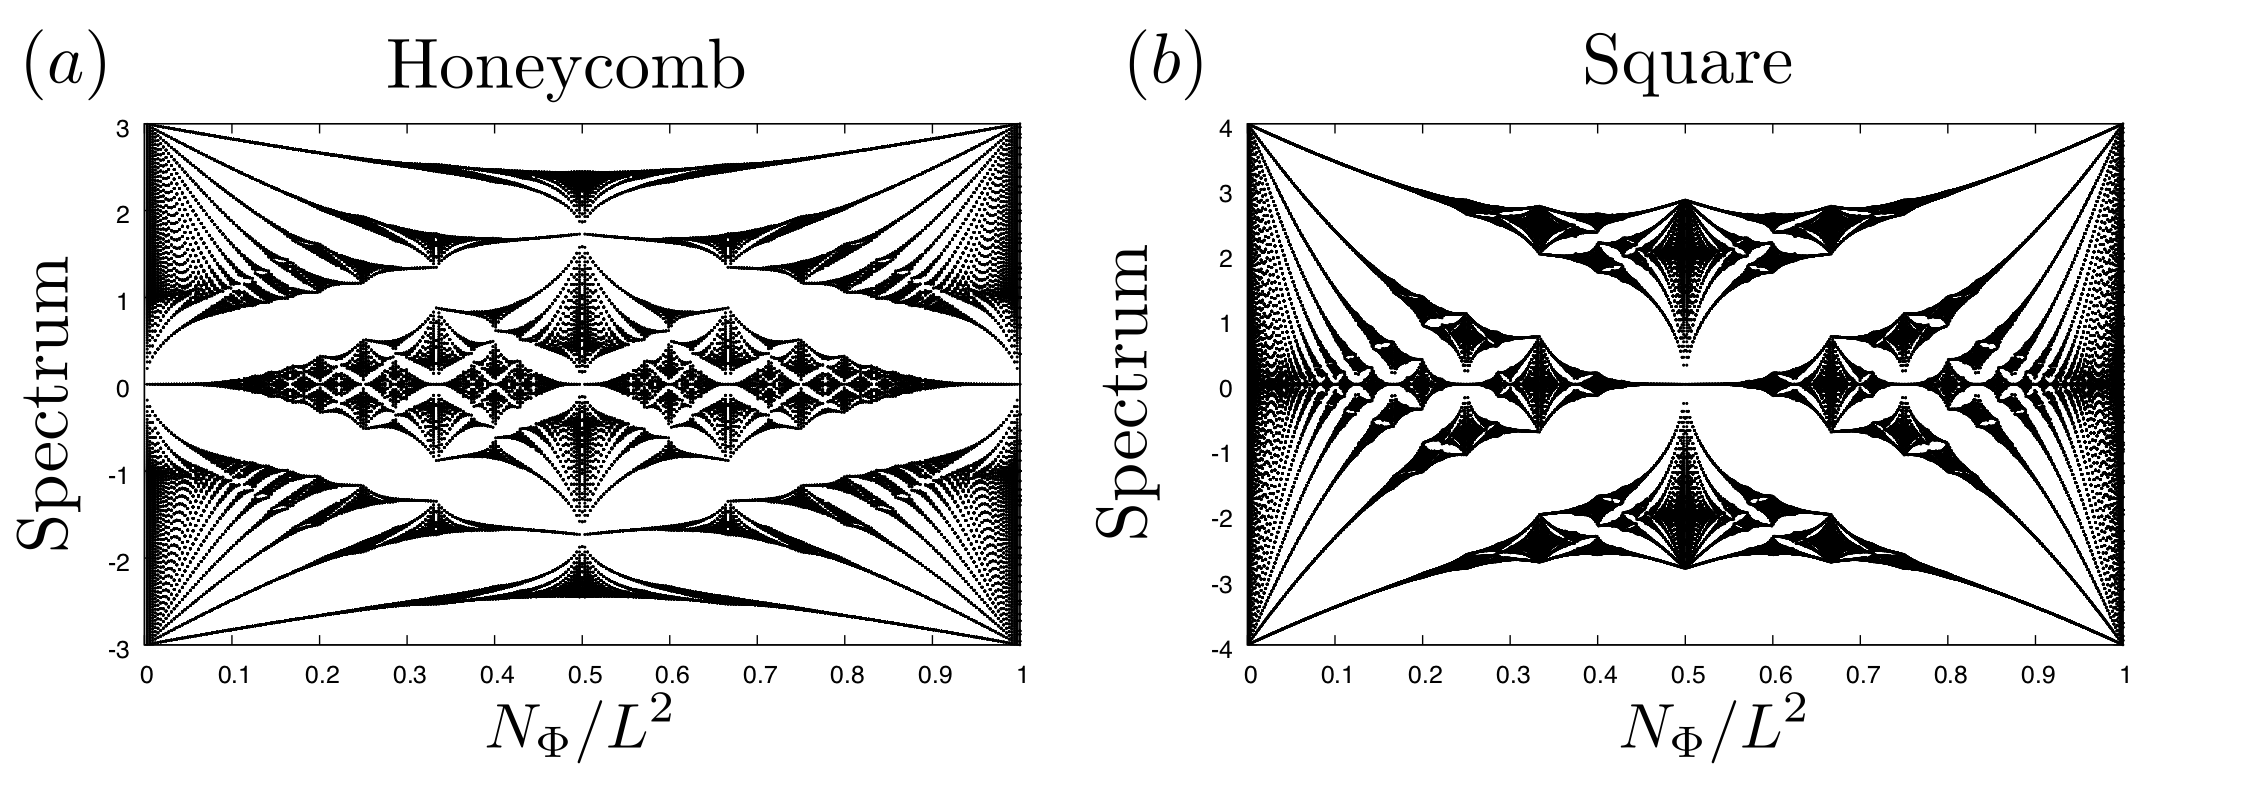
\includegraphics[width=0.95\textwidth,clip]{But.png}
		\caption{The single particle spectrum  of the tight binding model on the  honeycomb  (a) and square (b) lattices as a function of the  flux  $N_\Phi$.    This corresponds to the well known  Hofstadter butterflies.  }
		\label{But.fig}
	\end{center}
\end{figure}

For the honeycomb lattice of  Fig.~\ref{fig_predefined_lattices}(d)   the number of  bond within and emanating from  a unit cell is \texttt{N\_bonds = 3}.     The list array of the \texttt{Hopping\_matrix\_type} reads:

\begin{lstlisting}[style=fortran,escapechar=\#]
list(1,1) = 1;  list(1,2) = 2;  list(1,3) = 0;   list(1,4) =  0 ! Intra unit-cell hopping
list(2,1) = 2;  list(2,2) = 1;  list(2,3) = 0:   list(2,4) =  1 ! Inter unit-cell hopping
list(3,1) = 1;  list(3,2) = 2;  list(3,3) = 1:   list(3,4) = -1 ! Inter unit-cell hopping
T(1) = -1.0;  T(2) = -1.0;  T(3) = -1.0                         ! Hopping
T_loc(1) = 0.0;  T_loc(2) = 0.0                                 ! Chemical potential 
\end{lstlisting} 
In the last two lines, we have set the hopping matrix element  for each bond to $-1$  and the chemical potential to zero.    The fields,   can then be specified   with the  variables   \texttt{N\_phi, Phi\_x, Phi\_y}.  Setting   the twists, 
\texttt{Phi\_x, Phi\_y}  to zero and  looping over \texttt{N\_phi}    from $ 1 \cdots L^2 $   produces  the single particle spectrum of  Fig.~\ref{But.fig}(a).  

For the honeycomb lattice  the checkerboard decomposition  for the nearest neighbor hopping consists of three  sets:  \texttt{N\_Fam = 3}  each of length   corresponding  to the number of unit cells.  In  Fig.~\ref{fig_predefined_lattices}(d)  
these sets are denoted by different colors. In the code, the elements of the sets are specified as:

\begin{lstlisting}[style=fortran] 
do I = 1,Latt%N
   do nf = 1,N_FAM
      List_Fam(nf,I,1) = I  ! Unit cell
      List_Fam(nf,I,2) = nf ! The bond 
   enddo
enddo
Multiplicity  = 3
\end{lstlisting}        
Since each site of the honeycomb lattice occurs in  the three sets, their multiplicity is equal to 3.  


%-----------------------------------------------------------------------------------
\subsubsection{Predefined hoppings}

The  module provides hopping and checkerboard decompositions, defining a  \path{Hopping_Matrix} (an array of length \path{N_FL} of type  \path{Hopping_Matrix_type}, see Sec.~\ref{sec:hopping_type}) for each of the following predefined lattices.

\subsubsection*{Square}
The call:
\begin{lstlisting}[style=fortran]
Call Set_Default_hopping_parameters_square(Hopping_Matrix, T_vec, Chem_vec, Phi_X_vec,  
         Phi_Y_vec, Bulk, N_Phi_vec, N_FL, List, Invlist, Latt, Latt_unit)
\end{lstlisting}
defines  the  \path{Hopping_Matrix} for the square  lattice: 
\begin{equation}
\hat{H}_T  =   \sum_{\ve{i}, \sigma, s}  \left( \left[ \sum_{ \ve{\delta} = \left\{ \ve{a}_1, \ve{a}_2\right\} }    - t^{(s)} \hat{c}^{\dagger}_{\ve{i},s,\sigma}   e^{\frac{2 \pi i}{\Phi_0} \int_{\ve{i}}^{\ve{i}+ \ve{\delta}}  \vec{A}^{(s)}(\vec{l})  d \vec{l}}   \hat{c}^{}_{\ve{i} + \ve{\delta},s,\sigma} +  \hc   \right]    -  \mu^{(s)} \hat{c}^{\dagger}_{\ve{i},s,\sigma} \hat{c}^{}_{\ve{i},s,\sigma}  \right).
\end{equation}
The vectors  \path{T_vec} and \path{Chem_vec} have  length \texttt{N\_FL} and specify the hopping and the chemical potentials, while the  vectors \path{Phi_X_vec},  \path{Phi_Y_vec} and \path{N_Phi_vec},  also of  length  \texttt{N\_FL},    define the vector potential. 


\subsubsection*{Honeycomb}
The call: 
\begin{lstlisting}[style=fortran]
Call Set_Default_hopping_parameters_honeycomb(Hopping_Matrix,T_vec, Chem_vec, Phi_X_vec,
         Phi_Y_vec, Bulk, N_Phi_vec, N_FL, List, Invlist, Latt, Latt_unit)
\end{lstlisting}
defines  the  \path{Hopping_Matrix} for the  honeycomb lattice: 
\begin{align}
\hat{H}_T  &=  \sum_{\ve{i}, \sigma, s}  \left(  \sum_{ \ve{\delta} = \left\{ \ve{\delta}_1, \ve{\delta}_2, \ve{\delta}_3\right\} }    - t^{(s)} \hat{c}^{\dagger}_{\ve{i},s,\sigma}   e^{\frac{2 \pi i}{\Phi_0} \int_{\ve{i}}^{\ve{i}+ \ve{\delta}}  \vec{A}^{(s)}(\vec{l})  d \vec{l}}   \hat{c}^{}_{\ve{i} + \ve{\delta},s,\sigma} +  \hc \right)   \nonumber \\   
    &=  \sum_{\ve{i}, \sigma, s}   -  \mu^{(s)} \left( \hat{c}^{\dagger}_{\ve{i},s,\sigma} \hat{c}^{}_{\ve{i},s,\sigma}   +  \hat{c}^{\dagger}_{\ve{i} + \ve{\delta}_1,s,\sigma} \hat{c}^{}_{\ve{i} + \ve{\delta}_1,s,\sigma}   \right),
\end{align}
where the \path{T_vec} and \path{Chem_vec} have  length \texttt{N\_FL} and specify the hopping and the chemical potentials, while the  vectors \path{Phi_X_vec},  \path{Phi_Y_vec} and \path{N_Phi_vec},  also of  length  \texttt{N\_FL}, define the vector potential.  Here $\ve{i}$  runs over  sublattice  A, and $\ve{i} + \ve{\delta}$  over the three nearest neighbors of site $\ve{i}$.


\subsubsection*{Square bilayer}
The call:
\begin{lstlisting}[style=fortran]
Call Set_Default_hopping_parameters_Bilayer_square(Hopping_Matrix, T1_vec, T2_vec,
         Tperp_vec, Chem_vec, Phi_X_vec, Phi_Y_vec, Bulk, N_Phi_vec, N_FL, List, Invlist,
         Latt, Latt_unit)
\end{lstlisting}  
defines  the  \path{Hopping_Matrix} for the  bilayer  square  lattice:       
\begin{multline}
\hat{H}_T  =    \sum_{\ve{i}, \sigma, s,n } \left(    \left[  \sum_{ \ve{\delta} = \left\{ \ve{a}_1, \ve{a}_2\right\} } \!\! - t_n^{(s)} \hat{c}^{\dagger}_{\ve{i},s,\sigma,n}   e^{\frac{2 \pi i}{\Phi_0} \int_{\ve{i}}^{\ve{i}+ \ve{\delta}}  \vec{A}^{(s)}(\vec{l})  d \vec{l}}   \hat{c}^{}_{\ve{i} + \ve{\delta},s,\sigma,n} +  \hc \right]       -  \mu^{(s)} \hat{c}^{\dagger}_{\ve{i},s,\sigma,n} \hat{c}^{}_{\ve{i},s,\sigma,n}  \right)   \\
     + \sum_{\ve{i}, \sigma, s } -  t_{\perp}^{(s)}  \left( \hat{c}^{\dagger}_{\ve{i},s,\sigma,1} \hat{c}^{}_{\ve{i},s,\sigma,2}  + \hc \right), 
\end{multline}
where the additional  index  $n$  labels the layers.


\subsubsection*{Honeycomb  bilayer}
The call:
\begin{lstlisting}[style=fortran]
Call Set_Default_hopping_parameters_Bilayer_honeycomb(Hopping_Matrix, T1_vec, T2_vec,
         Tperp_vec, Chem_vec, Phi_X_vec, Phi_Y_vec, Bulk, N_Phi_vec, N_FL, List, Invlist,
         Latt, Latt_unit)
\end{lstlisting}  
defines  the  \path{Hopping_Matrix} for the  bilayer  honeycomb  lattice:                 
\begin{align}
\hat{H}_T  =  &   \sum_{\ve{i}, \sigma, s,n } \left(  \sum_{ \ve{\delta} = \left\{ \ve{\delta}_1, \ve{\delta}_2, \ve{\delta}_3 \right\} }  - t_n^{(s)} \hat{c}^{\dagger}_{\ve{i},s,\sigma,n}   e^{\frac{2 \pi i}{\Phi_0} \int_{\ve{i}}^{\ve{i}+ \ve{\delta}}  \vec{A}^{(s)}(\vec{l})  d \vec{l}}   \hat{c}^{}_{\ve{i} + \ve{\delta},s,\sigma,n} +  \hc \right)       \nonumber \\
      & +   \sum_{\ve{i}, \sigma, s } -  t_{\perp}^{(s)}  \left( \hat{c}^{\dagger}_{\ve{i},s,\sigma,1} \hat{c}^{}_{\ve{i},s,\sigma,2}   +
                   \hat{c}^{\dagger}_{\ve{i} + \ve{\delta}_1,s,\sigma,1} \hat{c}^{}_{\ve{i} + \ve{\delta}_1,s,\sigma,2}  + \hc  \right)   \nonumber \\
      & +   \sum_{\ve{i}, \sigma, s, n }  -  \mu^{(s)}  \left(\hat{c}^{\dagger}_{\ve{i},s,\sigma,n} \hat{c}^{}_{\ve{i},s,\sigma,n}  +  \hat{c}^{\dagger}_{\ve{i} + \ve{\delta}_1,s,\sigma,n} \hat{c}^{}_{\ve{i} + \ve{\delta}_1 ,s,\sigma,n}  \right)  
\end{align}
Here, the additional  index  $n$  labels the layer.   $\ve{i} $   runs over the unit cells  and   $\ve{\delta} = \left\{ \ve{\delta}_1, \ve{\delta}_2, \ve{\delta}_3 \right\} $  over the three nearest neighbors. 


\subsubsection*{N-leg ladder}
The call:
\begin{lstlisting}[style=fortran]
Call Set_Default_hopping_parameters_n_lag_ladder(Hopping_Matrix, T_vec, Tperp_vec,
    Chem_vec, Phi_X_vec, Phi_Y_vec, Bulk, N_Phi_vec, N_FL, List, Invlist, Latt, Latt_unit)
\end{lstlisting}  
defines  the  \path{Hopping_Matrix} for the  the  N-leg ladder lattice:                 
\begin{multline}
\hat{H}_T  =  \sum_{\ve{i}, \sigma, s }  \sum_{n=1}^{\texttt{Norb}} \left(      - t^{(s)} \hat{c}^{\dagger}_{\ve{i},s,\sigma,n}   e^{\frac{2 \pi i}{\Phi_0} \int_{\ve{i}}^{\ve{i}+ \ve{a}_1}  \vec{A}^{(s)}(\vec{l})  d \vec{l}}   \hat{c}^{}_{\ve{i} + \ve{a}_1,s,\sigma,n} +  \hc       -  \mu^{(s)} \hat{c}^{\dagger}_{\ve{i},s,\sigma,n} \hat{c}^{}_{\ve{i},s,\sigma,n}  \right)    \\
     + \sum_{\ve{i}, \sigma, s } \sum_{n=1}^{\texttt{Norb}-1}  -  t_{\perp}^{(s)}  \left( 
                   \hat{c}^{\dagger}_{\ve{i} + \ve{\delta}_1,s,\sigma,n}  e^{\frac{2 \pi i}{\Phi_0} \int_{(n-1)\ve{a}_2}^{(n)\ve{a}_2}  \vec{A}^{(s)}(\vec{l})  d \vec{l}}    \hat{c}^{}_{\ve{i} + \ve{\delta}_1,s,\sigma,n+1}  + \hc  \right). 
\end{multline}
Here, the additional  index  $n$  defines  the orbital.  Note that this lattice  has open boundary conditions in the $\vec{a}_2$  direction. 

%%%%%%%%%%%%%%%%%%%%%%%%%%%%

%%%%%%%%%%%%%%%%%%%%%%%%%%%%
% !TEX root = doc.tex
% Copyright (c) 2017-2020 The ALF project.
% This is a part of the ALF project documentation.
% The ALF project documentation by the ALF contributors is licensed
% under a Creative Commons Attribution-ShareAlike 4.0 International License.
% For the licensing details of the documentation see license.CCBYSA.
%
%-----------------------------------------------------------------------------------
\subsection{Predefined interaction vertices} \label{sec:interaction_vertices}
%-----------------------------------------------------------------------------------

In its most general form, an interaction Hamiltonian expressed in terms of sums of perfect squares can be written, as presented in Section~\ref{sec:intro}, as a sum of $M_V$ vertices: %Eq.~\eqref{eqn:general_ham_v}:

\begin{align*}
\hat{\mathcal{H}}_{V} &=  \sum\limits_{k=1}^{M_V}U_{k}
\left\{ \sum\limits_{\sigma=1}^{N_{\mathrm{col}}}
\sum\limits_{s=1}^{N_{\mathrm{fl}}} \left[ \left(
\sum\limits_{x,y}^{N_{\mathrm{dim}}} \hat{c}^{\dagger}_{x \sigma s}V_{xy}^{(k s)}\hat{c}^{\phantom\dagger}_{y \sigma s}\right)  +\alpha_{k s}  \right] \right\}^{2}
\equiv    \sum\limits_{k=1}^{M_V}U_{k}   \left(\hat{V}^{(k)} \right)^2 \tag{\ref{eqn:general_ham_v}}\\
&\equiv    \sum\limits_{k=1}^{M_V}\hat{\mathcal{H}}_V^{(k)},
\end{align*}
which are encoded in one or more variables of type \texttt{Operator}, described in Sec.~\ref{sec:op}. We often use arrays of \texttt{Operator} type, which should be initialized by repeatedly calling the subroutine \texttt{Op\_make}.

The module \texttt{Predefined\_Int\_mod.F90} implements some of the most common of such interaction vertices $\hat{\mathcal{H}}_V^{(k)}$, as detailed in the remaining of this section, where we drop the superscript $(k)$ when unambiguous.


\subsubsection{$SU(N)$ Hubbard interaction}
\label{Hubbard_SUN_HS.eq}
The $SU(N)$ Hubbard interaction on a given site $i$ is given by 
\begin{align}
%\label{eqn_hubbard_sun}
\hat{\mathcal{H}}_{V,i} =
+ \frac{U}{N_{\mathrm{col}}}\left[
\sum\limits_{\sigma=1}^{N_{\mathrm{col}}}
\left(  \hat{c}^{\dagger}_{i \sigma} \hat{c}^{\phantom\dagger}_{i\sigma}  -1/2 \right) \right]^{2}.
\end{align} 
Assuming that no other term in the Hamiltonian breaks the $SU(N) $ color symmetry, then this interaction term conveniently corresponds to  a single operator, obtained by calling, for each of the $N_{\mathrm{dim}}$ sites $i$:
\begin{lstlisting}[style=fortran]
Call Predefined_Int_U_SUN( OP, I, N_SUN, DTAU, U )
\end{lstlisting}
which defines:
%which corresponds to the general form of Eq.~\eqref{eqn:general_ham_v} by setting: 
%$N_{\mathrm{fl}} = 1$,  $M_V = N_{\text{unit-cell}} $,  $U_{k} =  -\frac{U}{N_{\mathrm{col}}}$,  $V_{x y}^{(ks)} =  \delta_{x,y} \delta_{x,k}$, and $\alpha_{ks} = -\frac{1}{2}$; and which is defined in the subroutine \texttt{Predefined\_Int\_U\_SUN} by a single operator:

\begin{lstlisting}[style=fortran]
Op%P(1)   = I
Op%O(1,1) = cmplx(1.d0,  0.d0, kind(0.D0))
Op%alpha  = cmplx(-0.5d0,0.d0, kind(0.D0))
Op%g      = SQRT(CMPLX(-DTAU*U/(DBLE(N_SUN)), 0.D0, kind(0.D0))) 
Op%type   = 2

\end{lstlisting}

To relate to  Eq.~\eqref{eqn:general_ham_v} we have,   $V_{x y}^{(is)} =  \delta_{x,y} \delta_{x,i}$, $\alpha_{is} = -\frac{1}{2}$ and $U_{k} =  \frac{U}{N_{\mathrm{col}}}$.   Here  the flavor index, $s$,  plays no role. 


\subsubsection{$M_z$-Hubbard interaction}

\begin{lstlisting}[style=fortran]
Call Predefined_Int_U_MZ( OP_up, Op_do, I, DTAU, U )
\end{lstlisting}

The $M_z$-Hubbard interaction is given by 
\begin{align}
%\label{eqn_hubbard_Mz}
\hat{\mathcal{H}}_{V} = - \frac{U}{2}\sum\limits_{i}\left[
\hat{c}^{\dagger}_{i \uparrow} \hat{c}^{\phantom\dagger}_{i \uparrow}  -   \hat{c}^{\dagger}_{i \downarrow} \hat{c}^{\phantom\dagger}_{i \downarrow}  \right]^{2},
\end{align} 
which corresponds to the general form of Eq.~\eqref{eqn:general_ham_v} by setting: 
$N_{\mathrm{fl}} = 2$, $N_{\mathrm{col}} \equiv \texttt{N\_SUN} =1 $,  $M_V =  N_{\text{unit-cell}} $,  $U_{k} = \frac{U}{2}$, 
$V_{x y}^{(i, s=1)} =  \delta_{x,y} \delta_{x,i}  $,  $V_{x y}^{(i, s=2)} =  - \delta_{x,y} \delta_{x,i}  $, and $\alpha_{is}   = 0  $; and which is defined in the subroutine \texttt{Predefined\_Int\_U\_MZ} by two operators:
\begin{lstlisting}[style=fortran]
Op_up%P(1)   = I
Op_up%O(1,1) = cmplx(1.d0, 0.d0, kind(0.D0))
Op_up%alpha  = cmplx(0.d0, 0.d0, kind(0.D0))
Op_up%g      = SQRT(CMPLX(DTAU*U/2.d0, 0.D0, kind(0.D0))) 
Op_up%type   = 2

Op_do%P(1)   = I
Op_do%O(1,1) = cmplx(1.d0, 0.d0, kind(0.D0))
Op_do%alpha  = cmplx(0.d0, 0.d0, kind(0.D0))
Op_do%g      = -SQRT(CMPLX(DTAU*U/2.d0, 0.D0, kind(0.D0))) 
Op_do%type   = 2

\end{lstlisting}


\subsubsection{$SU(N)$ $V$-interaction}

\begin{lstlisting}[style=fortran]
Call Predefined_Int_V_SUN( OP, I, J, N_SUN, DTAU, V )
\end{lstlisting}

The interaction term of the generalized t-V model, given by 
\begin{align}
\hat{\mathcal{H}}_{V,i,j} =
-\frac{V}{N_\mathrm{col}}\left[ \sum_{\sigma=1}^{N_\mathrm{col}}\left( \hat{c}^{\dagger}_{i \sigma} \hat{c}^{\phantom\dagger}_{j \sigma} + \hat{c}^{\dagger}_{j \sigma} \hat{c}^{\phantom\dagger}_{i \sigma} \right) \right]^2,
\end{align} 
is coded in the subroutine \texttt{Predefined\_Int\_V\_SUN} by a single symmetric operator:
\begin{lstlisting}[style=fortran]
Op%P(1)   = I
Op%P(2)   = J
Op%O(1,2) = cmplx(1.d0 ,0.d0, kind(0.D0)) 
Op%O(2,1) = cmplx(1.d0 ,0.d0, kind(0.D0))
Op%g      = SQRT(CMPLX(DTAU*V/real(N_SUN,kind(0.d0)), 0.D0, kind(0.D0))) 
Op%alpha  = cmplx(0.d0, 0.d0, kind(0.D0))
Op%type   = 2

\end{lstlisting}


\subsubsection{Fermion-Ising coupling}

\begin{lstlisting}[style=fortran]
Call Predefined_Int_Ising_SUN( OP, I, J, DTAU, XI )
\end{lstlisting}

The interaction between the Ising and a fermion degree of freedom, given by
\begin{align}
%\label{eqn_hubbard_sun_Ising}
\hat{\mathcal{H}}_{V,i,j} =
\hat{Z}_{i,j} \xi  \sum_{\sigma=1}^{N_\mathrm{col}}\left( \hat{c}^{\dagger}_{i \sigma} \hat{c}^{\phantom\dagger}_{j \sigma} + \hat{c}^{\dagger}_{j \sigma} \hat{c}^{\phantom\dagger}_{i \sigma} \right),
\end{align} 
where $\xi$ determines the coupling strength, is implemented in the subroutine \texttt{Predefined\_Int\_Ising\_SUN}:
\begin{lstlisting}[style=fortran]
Op%P(1)   = I
Op%P(2)   = J
Op%O(1,2) = cmplx(1.d0 ,0.d0, kind(0.D0)) 
Op%O(2,1) = cmplx(1.d0 ,0.d0, kind(0.D0)) 
Op%g      = cmplx(-DTAU*XI,0.D0,kind(0.D0))
Op%alpha  = cmplx(0d0,0.d0, kind(0.D0)) 
Op%type   = 1

\end{lstlisting}



\subsubsection{Long-Range Coulomb repulsion}

\begin{lstlisting}[style=fortran]
Call Predefined_Int_LRC( OP, I, DTAU )
\end{lstlisting}

The Long-Range Coulomb (LRC) interaction can be written as
\begin{align}
\hat{\mathcal{H}}_{V} =
\frac{1} { N } \sum_{\vec{i},\vec{j}}  \left(  \hat{n}_{i} -  \frac{N}{2}  \right)  V_{i,j} \left(  \hat{n}_{j} -  \frac{N}{2}  \right), 
\end{align} 
where
\begin{align}
\hat{n}_{i} = \sum_{\sigma=1}^{N}  \hat{c}^{\dagger}_{i,\sigma}  \hat{c}^{}_{i,\sigma}
\end{align} 
and  $i$ corresponds to a super-index labelling  the unit cell and orbital. 


  The code uses the following  HS decomposition:
\begin{equation}
e^{-\Delta \tau \hat{H}_{V,k} }  =  \int \prod_{\vec{i}} d \phi_{i}   e^{ - \frac{N \Delta \tau} {4} \phi_{i} V^{-1}_{i,j}  \phi_{j} - \sum_{i}  i \Delta \tau \phi_i \left( \hat{n}_{i} - \frac{N}{2} \right) }.
\end{equation}
The above holds only provided that the matrix $V$ is positive definite and the implementation follows Ref.~\cite{Hohenadler14}.   

The LRC interaction is implemented in the subroutine \texttt{Predefined\_Int\_LRC}:
\begin{lstlisting}[style=fortran]
Op%P(1)   = I
Op%O(1,1) = cmplx(1.d0  ,0.d0, kind(0.D0))
Op%alpha  = cmplx(-0.5d0,0.d0, kind(0.D0))
Op%g      = cmplx(0.d0  ,DTAU, kind(0.D0)) 
Op%type   = 3
\end{lstlisting}


\subsubsection{$J_z$-$J_z$ interaction}

\begin{lstlisting}[style=fortran]
Call Predefined_Int_Jz( OP_up, Op_do, I, J, DTAU, Jz )
\end{lstlisting}

Another predefined vertex is:
\begin{align}
\hat{\mathcal{H}}_{V,i,j} =
- \frac{|J_z|}{2}  \left( S^{z}_i - \sgn|J_z| S^{z}_j \right)^2 =
J_z  S^{z}_i  S^{z}_j  - \frac{|J_z|}{2} (S^{z}_i)^2 - \frac{|J_z|}{2}(S^{z}_j)^2 
\end{align} 
which, if particle fluctuations are frozen on the $i$ and $j$ sites, then $(S^{z}_i)^2 = 1/4$ and the interactions corresponds to a 
$J_z$-$J_z$ ferromagnetic or antiferromagnetic coupling.

The implementation of the interaction in \texttt{Predefined\_Int\_Jz} defines two operators:
\begin{lstlisting}[style=fortran]
Op_up%P(1)   = I
Op_up%P(2)   = J
Op_up%O(1,1) = cmplx(1.d0,              0.d0, kind(0.D0))
Op_up%O(2,2) = cmplx(-Jz/Abs(Jz),       0.d0, kind(0.D0))
Op_up%alpha  = cmplx(0.d0,              0.d0, kind(0.D0))
Op_up%g      = SQRT(CMPLX(DTAU*Jz/8.d0, 0.d0, kind(0.D0))) 
Op_up%type   = 2

Op_do%P(1)   = I
Op_do%P(2)   = J
Op_do%O(1,1) = cmplx(1.d0,               0.d0, kind(0.d0))
Op_do%O(2,2) = cmplx(-Jz/Abs(Jz),        0.d0, kind(0.d0))
Op_do%alpha  = cmplx(0.d0,               0.d0, kind(0.d0))
Op_do%g      = -SQRT(CMPLX(DTAU*Jz/8.d0, 0.d0, kind(0.d0))) 
Op_do%type   = 2

\end{lstlisting}

%%%%%%%%%%%%%%%%%%%%%%%%%%%%

%%%%%%%%%%%%%%%%%%%%%%%%%%%%
% Copyright (c) 2016-2020 The ALF project.
% This is a part of the ALF project documentation.
% The ALF project documentation by the ALF contributors is licensed
% under a Creative Commons Attribution-ShareAlike 4.0 International License.
% For the licensing details of the documentation see license.CCBYSA.

% !TEX root = doc.tex

\subsection{Predefined trial wave functions} \label{sec:predefined_trial_wave_function}

When using the projective algorithm (see Sec.~\ref{sec:defT0}), trial wave functions must be specified.
These are stored in variables of the \texttt{WaveFunction} type (Sec.~\ref{sec:wave_function}).
The ALF package provides a set of predefined trial wave functions $|\Psi_{T,L/R}\rangle$=\texttt{WF\_L/R}, returned by the call:

\begin{lstlisting}[style=fortran]
Call Predefined_TrialWaveFunction(Lattice_type, Ndim, List, Invlist, Latt, Latt_unit, N_part,
                                  N_FL, WF_L, WF_R)
\end{lstlisting}
Twisted boundary conditions (\texttt{Phi\_X\_vec=0.01}) are implemented for some lattices so as to generate a non-degenerate trial wave function. Here the marker "\texttt{\_vec}" indicates the variable may assume different values depending on the flavor (e.g., spin up and down). Currently predefined trial wave functions are flavor independent.

The predefined trial wave functions correspond to the solution of the non-interacting tight binding Hamiltonian on each of the predefined lattices. These solutions are the ground states of the predefined hopping matrices (Sec.~\ref{sec:predefined_hopping}) with default parameters, for each lattice, as follows.

\subsubsection{Square}

Parameter values for the predefined trial wave function on the square lattice:
\begin{lstlisting}[style=fortran]
Checkerboard  = .false.
Symm          = .false.
Bulk          = .false.
N_Phi_vec     = 0
Phi_X_vec     = 0.01d0
Phi_Y_vec     = 0.d0
Ham_T_vec     = 1.d0
Ham_Chem_vec  = 0.d0
Dtau          = 1.d0
\end{lstlisting}
%Ham_T2_vec    = 0.d0
%Ham_Tperp_vec = 0.d0


\subsubsection{Honeycomb}

\red{[JSEP: I'm not sure how to best describe the definition of the trial wave function for the honeycomb, since it doesn't use the Predefined Hopping module.\\
	  Also, do we want to mention the \texttt{Kekule\_Trial} option?]}\\
Parameter values for the predefined trial wave function on the Honeycomb lattice:
\begin{lstlisting}[style=fortran,escapechar=\#]
Checkerboard  = .false.
Symm          = .false.
Bulk          = .false.
N_Phi_vec     = 0
Phi_X_vec     = 0.d0
Phi_Y_vec     = 0.d0
Ham_T_vec     = 1.d0
Ham_Tperp_vec = 0.d0
Ham_Chem_vec  = 0.d0
Dtau          = 1.d0
\end{lstlisting}
%delta         = 0.01d0
%Kekule_Trial  = .false. #\red{(include?)}#
%Ham_T2_vec    = 0.d0


\subsubsection{N-leg ladder}

Parameter values for the predefined trial wave function on the N-leg ladder lattice:
\begin{lstlisting}[style=fortran]
Checkerboard  = .false.
Symm          = .false.
Bulk          = .false.
N_Phi_vec     = 0
Phi_X_vec     = 0.01d0
Phi_Y_vec     = 0.d0
Ham_T_vec     = 1.d0
Ham_Tperp_vec = 1.d0
Ham_Chem_vec  = 0.d0
Dtau          = 1.d0
\end{lstlisting}
%Ham_T2_vec    = 0.d0


\subsubsection{Bilayer square}

Parameter values for the predefined trial wave function on the bilayer square lattice:
\begin{lstlisting}[style=fortran]
Checkerboard  = .false.
Symm          = .false.
Bulk          = .false.
N_Phi_vec     = 0
Phi_X_vec     = 0.d0
Phi_Y_vec     = 0.d0
Ham_T_vec     = 1.d0
Ham_T2_vec    = 0.d0
Ham_Tperp_vec = 1.d0
Ham_Chem_vec  = 0.d0
Dtau          = 1.d0
\end{lstlisting}


\subsubsection{Bilayer honeycomb}

Parameter values for the predefined trial wave function on the bilayer honeycomb lattice:
\begin{lstlisting}[style=fortran]

Checkerboard  = .false.
Symm          = .false.
Bulk          = .false.
N_Phi_vec     = 0
Phi_X_vec     = 0.d0
Phi_Y_vec     = 0.d0
Ham_T_vec     = 1.d0
Ham_T2_vec    = 0.d0
Ham_Tperp_vec = 1.d0
Ham_Chem_vec  = 0.d0
Dtau          = 1.d0
\end{lstlisting}


%%%%%%%%%%%%%%%%%%%%%%%%%%%%


\subsection{Template}

\red{Maybe discard this subsection.}\\
	
\red{Maybe merge this with Chapter on Examples and Models/Model Classes.\\}

 \red{TODO} Go through everything one has to defined/set in order to define a new Hamiltonian. \red{TODO}\\

We'd perhaps want to provide a \emph{minimum} Hamiltonian, probably written in pseudo-code, from which one could write their own.\\ \\

\noindent A \emph{complete} list of all the code that would have to be changed for the \emph{most general} case could read as:

\begin{itemize}
	\item Hamiltonian -- one-body, imaginary-time propagator for a given configuration of HS and  Ising fields
	\item Table~\ref{table:hamiltonian}:
	\begin{itemize}
		\item \texttt{Ham\_Set}
		\item \texttt{Ham\_V}
		\item \texttt{S0}
		\item \texttt{Setup\_Ising\_action}
		\item \texttt{Global\_move}
		\item \texttt{Delta\_S0\_global}
		\item \texttt{Global\_move\_tau}
		\item \texttt{Alloc\_obs}
		\item \texttt{Obser}
		\item \texttt{ObserT}
	\end{itemize}
	\item Check Table~\ref{table:operator} (Operator type).
	\item Table~\ref{table:lattice} and \ref{table:unit_cell}:
	\begin{itemize}
		\item \texttt{Lattice\%a1\_p}, \texttt{Lattice\%a2\_p}
		\item \texttt{Lattice\%L1\_p}, \texttt{Lattice\%L2\_p}
		\item \texttt{Lattice\%N}
		\item \texttt{Norb}
		\item \texttt{N\_coord}
		\item \texttt{Orb\_pos(1..Norb,2)}
	\end{itemize}
\end{itemize}

